\section{Trapezregel}
\label{sec:trapezregel}

\subsection{Herleitung}
\label{sec:herleitung}

\begin{figure}[h]
    \centering
    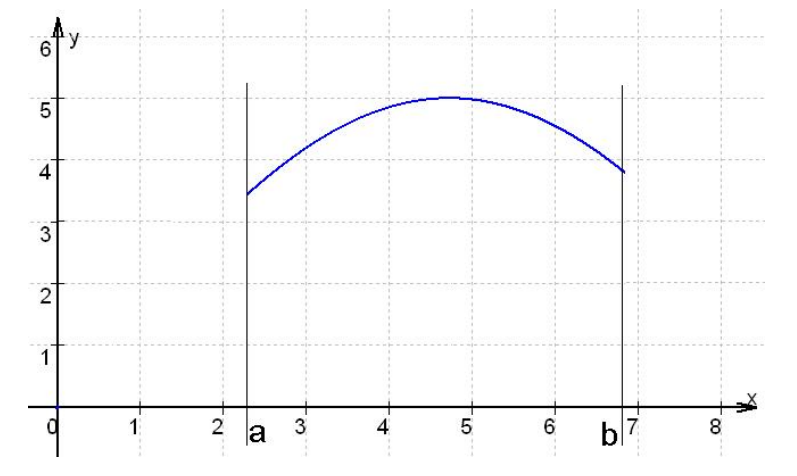
\includegraphics[width=8cm]{Bilder/keplersche_fassregel_funktion.png}
    \caption{Keplersche Fassregel \cite{skript}}    
    \label{fig:keplersche_fassregel}
\end{figure}

Wir betrachten eine Funktion $f$, deren Schaubild im gewünschten Intervall $I = [a, b]$ in \autoref{fig:sehnentrapeze} gezeigt ist.

\begin{figure}[!tbp]
    \centering
    \begin{minipage}[b]{0.4\textwidth}
        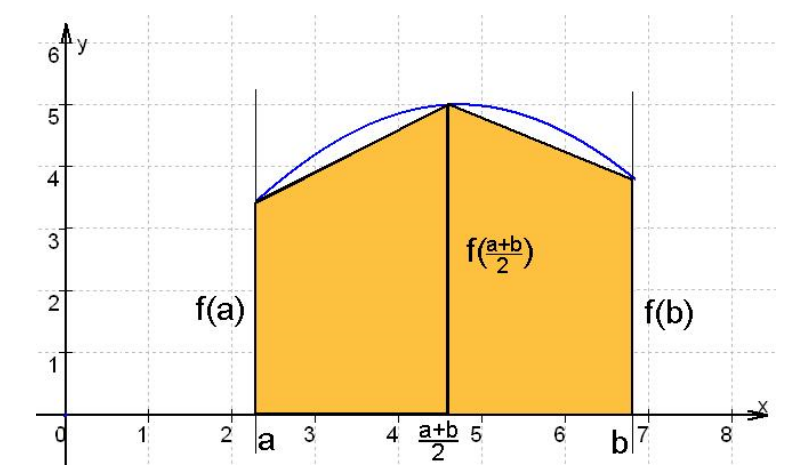
\includegraphics[width=8cm]{Bilder/sehnentrapeze.png}
      \caption{Sehnentrapeze für die anstehende Rechnung}
    \end{minipage}
    \hfill
    \begin{minipage}[b]{0.4\textwidth}
        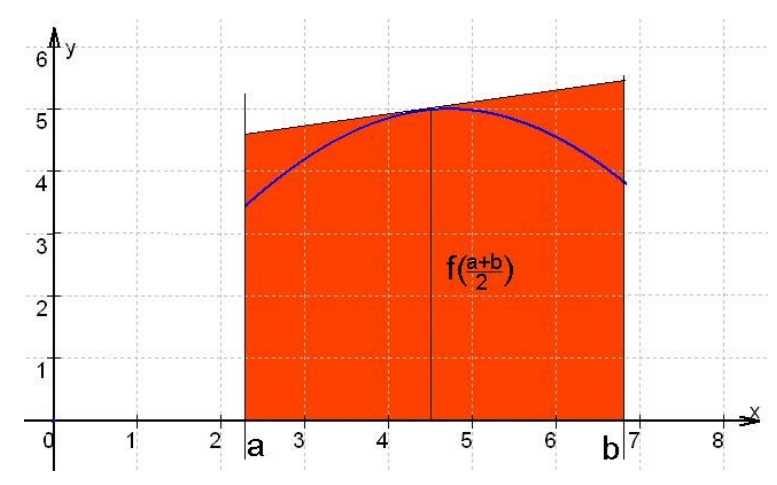
\includegraphics[width=8cm]{Bilder/sehnentrapez_addiert.png}
      \caption{Tangententrapez  \cite{skript}}
    \end{minipage}
    \label{fig:sehnentrapeze}
  \end{figure}
\subsection*{A. Die zwei Sehnentrapeze}

Zur Flächenberechnung zeichnen wir zwei Sehnentrapeze in das gegebene Schaubild, wie in \autoref{fig:sehnentrapeze} zu sehen ist. Für die Fläche eines Trapezes gilt:
\[
A_{\text{Trapez}} = \frac{a + c}{2} \cdot h = m \cdot h
\]
Übertragen auf die beiden Sehnentrapeze ergibt sich die Gesamtfläche $S$ als:
\[
S = \frac{b - a}{2} \cdot \left(\frac{f(a)}{2} + f\left(\frac{a + b}{2}\right) + \frac{f(b)}{2}\right)
\]
Dies lässt sich umschreiben zu:
\[
S = \frac{b - a}{2} \cdot \left(\frac{f(a)}{2} + f\left(\frac{a + b}{2}\right) + \frac{f(b)}{2}\right)
\]

\subsection*{B. Das Tangententrapez}

Nun legen wir ein weiteres Tangententrapez in das Schaubild, wie in \autoref{fig:sehnentrapeze} dargestellt. Nach der Trapezformel ergibt sich:
\[
T = f\left(\frac{a + b}{2}\right) \cdot (b - a)
\]
Da wir doppelt so viele Sehnentrapeze wie Tangententrapeze haben, gewichten wir die Flächen entsprechend. Die Gesamtfläche $I[f]$ nähert sich durch:
\[
I[f] \approx A = \frac{1}{3} \cdot (2S + T)
\]
Dies lässt sich weiter vereinfachen zu:
\[
A = \frac{b - a}{6} \cdot \left(f(a) + 4 \cdot f\left(\frac{a + b}{2}\right) + f(b)\right)
\]

\subsection*{Die Keplersche Fassregel}

Ist die Funktion $f$ auf dem Intervall $I = [a, b]$ stetig, so gilt die Keplersche Fassregel:
\[
I[f] \approx A = \frac{b - a}{6} \cdot \left(f(a) + 4 \cdot f\left(\frac{a + b}{2}\right) + f(b)\right)
\]
Dabei ist zu beachten, dass die Keplersche Fassregel nur dann gute Näherungswerte liefert, wenn sich die Funktion im betrachteten Intervall durch eine Parabel annähern lässt. Daher ist es ratsam, das Intervall $[a, b]$ in viele kleine, gleich große Teilintervalle zu unterteilen und die Keplersche Fassregel auf jedes Teilintervall anzuwenden. Diese Methode wird im nächsten Abschnitt besprochen, in dem die summierten Regeln behandelt werden. \cite{skript}

\subsection{Fehlerabschätzung}
\label{sec:fehlerabschätzung}

\subsection{Vertrauensniveau $\gamma$}
\label{sec:vertrauensniveau}

\subsection{Alternativen zur Trapezregel} 
\label{sec:alternativen}
